\section{Linealización en hover y evidencia de que el modelo no lineal la recupera}
\label{sec:linealizacion}

La linealización en vuelo estacionario no se usa para simular: el
simulador integra siempre el modelo completo. Se usa para dos cosas. Para
\emph{diseñar} controladores (las reglas SIMC de la \cref{sec:control} y el
MPC lineal de la \cref{sec:posicion} parten de ella), y para \emph{verificar}
el código: si el modelo no lineal está bien programado, su jacobiano numérico
en hover tiene que coincidir con las derivadas analíticas, y su respuesta a
ángulos pequeños tiene que coincidir con la del modelo lineal.

\subsection{Punto de equilibrio}

Con $\vect v=\vect0$, $\vect q=(1,0,0,0)$, $\vect\omega=\vect 0$,
$\Omega_i=\Omega_h$ y $\sigma_i=\sigma_h$ de \eqref{eq:hover}, todas las
derivadas de \eqref{eq:newton}--\eqref{eq:rotor} se anulan. El residuo
numérico de \cod{derivative} en ese punto es $\max|\dot{\vect x}|=\val{resHover}$,
y diez segundos de integración RK4 en lazo abierto desde el equilibrio
terminan con una velocidad de $\val{driftV}$~m/s: el equilibrio es exacto
hasta el redondeo. El acelerómetro ideal mide en ese estado $(0,0,-g)$.

\subsection{Modelo linealizado}

Con ángulos pequeños, $\vect q\approx(1,\phi/2,\theta/2,\psi/2)$ y
$\R\approx I+\sk{(\phi,\theta,\psi)}$. Escribiendo
$\delta\Omega_i=\Omega_i-\Omega_h$ y $\delta\sigma_i=\sigma_i-\sigma_h$:
\begin{align}
\dot v_x &= -g\,\theta, \qquad \dot v_y = g\,\phi, \qquad
\dot v_z = -\frac{2C_T\Omega_h}{m}\sum_i\delta\Omega_i, \label{eq:lin_tras}\\
\dot\phi &= p,\qquad \dot\theta=q,\qquad \dot\psi=r, \label{eq:lin_cin}\\
\dot p &= \frac{2C_T\Omega_h}{J_{xx}}\sum_i(-y_i)\,\delta\Omega_i,\quad
\dot q = \frac{2C_T\Omega_h}{J_{yy}}\sum_i x_i\,\delta\Omega_i,\quad
\dot r = \frac{2C_M\Omega_h}{J_{zz}}\sum_i e_i\,\delta\Omega_i, \label{eq:lin_rot}\\
T_m\,\delta\dot\Omega_i &= C_R\,\delta\sigma_i - \delta\Omega_i. \label{eq:lin_mot}
\end{align}
Desaparecen tres familias de términos. $\vect\omega\times J\vect\omega$ y el
amortiguamiento $C_{Cm}\omega|\omega|$ son de segundo orden en $\vect\omega$;
el término giroscópico se anula porque en hover $h_z=0$ (dos rotores giran
en cada sentido a la misma velocidad); el arrastre cuadrático tiene
derivada nula en $\vect v=\vect0$. Lo que queda es la estructura que justifica
la cascada de control: cada eje angular es un doble integrador detrás de un
primer orden (el motor), y la traslación horizontal es otro doble integrador
cuya entrada es el ángulo. Powers, Mellinger y Kumar \cite{hb16} (pp.~318--319)
lo dicen en una frase: en ángulos pequeños las aceleraciones angulares
están desacopladas, cada una depende solo de su componente de momento.

\subsection{Jacobiano numérico contra derivadas analíticas}

El bloque D calcula por diferencias centrales el jacobiano $\partial\dot{\vect x}/\partial\vect x$
del modelo completo en hover y lo compara con \eqref{eq:lin_tras}--\eqref{eq:lin_rot}:

\begin{table}[H]
\centering
\small
\caption{Jacobiano del modelo no lineal en hover frente a la linealización analítica.}
\label{tab:jac}
\begin{tabular}{lll}
\toprule
Derivada & Numérica (modelo completo) & Analítica \\
\midrule
$\partial\dot v_y/\partial\phi$, $\partial\dot v_x/\partial\theta$ & $9.80665$, $-9.80665$ & $g$, $-g$ \\
$\partial\dot v_z/\partial\Omega_i$ [m/s$^2$ por rad/s] & \val{dvzdO} & $-2C_T\Omega_h/m$, idéntico a 10 cifras \\
$\partial\dot p/\partial\Omega_i$ (M1, M2, M3, M4) & $\mp\val{dpdO}$ con signos $(-,+,+,-)$ & $-y_i\,2C_T\Omega_h/J_{xx}$ \\
$\partial\dot r/\partial\Omega_i$ & $\pm\val{drdO}$ con signos $(+,+,-,-)$ & $e_i\,2C_M\Omega_h/J_{zz}$ \\
$\max|\partial\dot{\vect\omega}/\partial\vect\omega|$ & \val{cross} & 0 \\
Autovalores & 13 nulos y cuatro en \val{eigMin} & 0 y $-1/T_m=-50$ \\
\bottomrule
\end{tabular}
\end{table}

\subsection{Ganancia de planta del lazo de tasa}

Para el diseño del lazo de tasa interesa la ganancia entre el momento
normalizado $u$ y la aceleración angular. De \eqref{eq:lin_rot} y del
mezclador, en régimen,
\begin{equation}
\frac{\dot p}{u} = K_x = \frac{\tau_{x,max}}{J_{xx}} = \val{Kpred}~\text{rad/s}^2 .
\label{eq:Krate}
\end{equation}
Aplicando un escalón $u=0.02$ al modelo completo a través del mezclador real,
la ganancia medida es \val{Kmed1} a los 0.1~s (cinco constantes de tiempo
del motor) y \val{Kmed2} a los 0.2~s. La diferencia de 1--1.4~\% es el
amortiguamiento rotacional \eqref{eq:damp}, que crece con la velocidad
angular que el propio escalón produce y que la linealización elimina. A
$t=T_m$ la respuesta va en el \val{fracTm} de su valor final, frente al
$1-e^{-1}=0.632$ de un primer orden: el motor del modelo completo se comporta
como dice \eqref{eq:lin_mot}.

\subsection{Lazo cerrado: no lineal frente a linealizado}

La prueba más exigente compara las dos plantas dentro del simulador
completo, con el mismo controlador. El bloque F reemplaza la planta por
una clase \cod{HoverLinearDynamics} que implementa
\eqref{eq:lin_tras}--\eqref{eq:lin_mot} con el mismo vector de estado, y
aplica escalones de roll de 2, 5, 15 y 30$^\circ$ de 0.5~s, con estimador
ideal y sensores sin ruido (para aislar la dinámica).

\begin{table}[H]
\centering
\small
\caption{Diferencia máxima entre la planta no lineal y la linealizada en
lazo cerrado, ante escalones de roll de 0.5~s.}
\label{tab:linnl}
\begin{tabular}{rcccc}
\toprule
Escalón & $\max|\Delta\phi|$ [$^\circ$] & relativo al escalón & $\max|\Delta y|$ [cm] (desplazamiento) & $\max|\Delta h|$ [cm] \\
\midrule
2$^\circ$  & \val{F2phi}  & \val{F2rel}~\%  & \val{F2y} (de \val{F2ymax}~m)  & \val{F2h} \\
5$^\circ$  & \val{F5phi}  & \val{F5rel}~\%  & \val{F5y} (de \val{F5ymax}~m)  & \val{F5h} \\
15$^\circ$ & \val{F15phi} & \val{F15rel}~\% & \val{F15y} (de \val{F15ymax}~m) & \val{F15h} \\
30$^\circ$ & \val{F30phi} & \val{F30rel}~\% & \val{F30y} (de \val{F30ymax}~m) & \val{F30h} \\
\bottomrule
\end{tabular}
\end{table}

\begin{figure}[H]
\centering
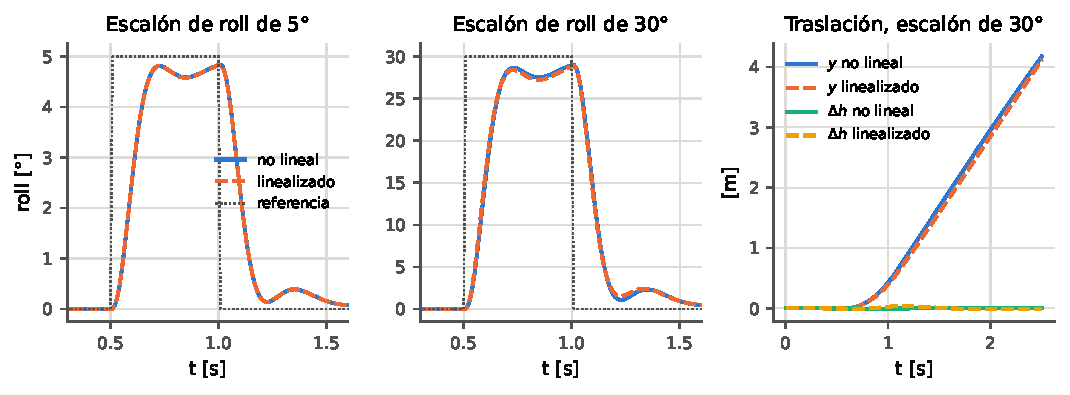
\includegraphics[width=\textwidth]{lineal_vs_no_lineal.pdf}
\caption{Lazo cerrado con la planta no lineal y con la linealizada en hover.
Izquierda y centro: escalones de roll de 5$^\circ$ y 30$^\circ$. Derecha:
desplazamiento lateral y cambio de altura durante el escalón de 30$^\circ$.}
\label{fig:linnl}
\end{figure}

La lectura es la esperada y, por eso, informativa. Hasta 5$^\circ$ las dos
plantas son indistinguibles (diferencias del \val{F2rel} y \val{F5rel}~\%); a
15$^\circ$ la diferencia en roll es del \val{F15rel}~\% y a 30$^\circ$ del
\val{F30rel}~\%, y aparece sobre
todo en la vuelta a cero, donde la proyección $\cos\phi$ del empuje y el
acoplamiento con la altura empiezan a pesar. El modelo no lineal recupera
la linealización en su dominio de validez, y se separa de ella de forma
gradual y con el signo correcto fuera de él. Que la 3.ª edición use el
modelo completo importa justamente en la figura en 8 rápida
(\cref{sec:posicion}), con inclinaciones de hasta \val{lemRTilt}$^\circ$.
